\documentclass[12pt,a4paper]{article}
\usepackage{amsmath,amssymb}
\usepackage{eso-pic}
\usepackage[most]{tcolorbox}
\usepackage{pgfplots}
\pgfplotsset{compat=1.18}
\newtcolorbox{solution}[1]{enhanced,breakable,colback=gray!10,
  colframe=gray!60!black,title={#1},fonttitle=\bfseries}
\pagestyle{empty}
\setlength{\unitlength}{1bp}
\setlength{\parindent}{0pt}

% Position a text paragraph; its contents remain ordinary editable LaTeX.
\newcommand{\TextAt}[4]{%
  \put(#1bp,-#2bp){\vtop{%
    \hsize=#3bp\relax
    \parindent=0pt\relax
    \parskip=0pt\relax
    \baselineskip=23.9975pt\relax
    \noindent#4\par}}}
\newcommand{\At}[3]{\put(#1bp,-#2bp){#3}}
\newcommand{\MathAt}[3]{\At{#1}{#2}{$\displaystyle #3$}}
\newcommand{\EquationNumber}[2]{\At{513.865}{#1}{(I.#2)}}
\newcommand{\PageFurniture}[1]{%
  \At{62.362}{58.290}{Problem Set 2}%
  \At{332.179}{58.290}{Physics286/AP286/MCB 198 Fall-2026}%
  \At{62.362}{63.022}{\rule{470.551bp}{0.398bp}}%
  \At{294.711}{800.912}{#1}}
\newcommand{\SourcePage}[2]{%
  \AddToShipoutPictureFG*{\AtPageUpperLeft{%
    \PageFurniture{#1}%
    #2}}%
  \null\newpage}

\begin{document}

% =========================== PAGE 1 ===========================
\SourcePage{1}{%
  \At{240.174}{128.126}{{\LARGE Problem set 2}}
  \At{65.749}{356.983}{\textbf{Problem 1. Double Descent. Optional for MCB198}}
  \At{77.393}{380.891}{\textbf{a)}}
  \TextAt{95.014}{380.891}{441.286}{%
    write code to generate ten data points $\{(x,y)\}$ between $0\leq x\leq 1$, $y(x)=a*x+\eta$
    where $\eta$ is a Gaussain distributed random variable with mean 0 and variance 1.}

  \At{76.459}{434.559}{\textbf{b)}}
  \TextAt{95.014}{434.559}{441.286}{%
    Set $a=0$ above and generate the K=10 data points. Fit this data to the first N terms
    of the Fourier series that minimizes}
  \MathAt{208.375}{506.283}{%
    \mathcal{L}(\mathbf{a})=
    \sum_{i=1}^{K}\left|y_i-\sum_{k=0}^{N-1}a_ke^{ikx_i}\right|^2
    +\lambda\sum_{k=0}^{N-1}|a_k|^2}
  \EquationNumber{506.283}{1}
  \TextAt{95.014}{540.908}{441.286}{%
    Where the second term as will be described in class arises from a Gaussian Prior on
    the coefficients, and is called the $L_2$ norm. Do this over a range of $N$ and $\lambda$.}

  \At{77.953}{594.577}{\textbf{c)}}
  \TextAt{95.014}{594.577}{441.286}{%
    Generate several more K=10 sets of data points from the same generative model to
    calculate the generalization error. Calculate the error in the fit to these new data
    points and plot the average generalization error as a function of $N$. Discuss how the
    generalization error changes as a function of N and look for parameter values $\lambda$ for
    which for very large $N$ you start seeign the double descent phenomena as described in
    class. Discuss why the double descent happens for this simple problem.}
}

% =========================== PAGE 2 ===========================
\SourcePage{2}{%
  \At{65.749}{96.729}{\textbf{Problem 2. Gamma Function and $N!$ for large $N$}}
  \At{65.749}{120.637}{Start with the result}
  \MathAt{257.387}{144.545}{\int_0^\infty dxe^{-\alpha x}=\frac{1}{\alpha}.}
  \EquationNumber{144.545}{2}

  \TextAt{65.749}{179.170}{470.551}{%
    Differentiate this equation $N$ times with respect to $\alpha$ and then set $\alpha=1$ to show that}
  \MathAt{250.766}{222.863}{N!=\int_0^\infty dxx^Ne^{-x}.}
  \EquationNumber{222.863}{3}

  \TextAt{65.749}{266.557}{470.551}{%
    This function is also known as the $\Gamma$ function and $N!=\Gamma(N+1)$. Using integration through
    Saddle Point integration show that:}
  \MathAt{208.654}{334.158}{\log N!=N\log N-N+\frac{1}{2}\log(2\pi N)}
  \EquationNumber{334.158}{4}
}

% =========================== PAGE 3 ===========================
\SourcePage{3}{%
  \At{65.749}{96.729}{\textbf{Problem 3}}
  \TextAt{65.749}{120.637}{470.551}{%
    One important task in motor control is tracking. We do this in many situations, but when
    objects move smoothly across our visual field, we track their motion by moving our eyes.
    This behavior is called smooth pursuit.}
  \TextAt{95.014}{192.360}{441.286}{%
    (a) The simplest version of the tracking problem is that we have an observable $x$ and
    we try to generate a variable $y$ that is as close as possible to $x$. Assume that $x$ is chosen
    out of a distribution $P\left(x\right)$ and that 'as close as possible' will be measured by the mean-squared error,
    $\epsilon=\left\langle\left(y-x\right)^2\right\rangle$. Develop a variational problem to find the minimum
    amount of mutual information $I\left(y,x\right)$ required, and the associated distribution $P\left(y|x\right)$,
    to reach a value of $\epsilon$.}
  \TextAt{95.014}{335.807}{441.286}{%
    (b) Show that the variational problem you formulated in part (a) is solved by}
  \MathAt{207.192}{379.501}{%
    P\left(y|x\right)=\frac{1}{Z\left(x,\beta\right)}P\left(y\right)
    \exp\left[-\beta\left(y-x\right)^2\right],}
  \At{95.014}{423.195}{where $\beta$ is a parameter, and}
  \MathAt{213.493}{466.888}{%
    Z\left(x,\beta\right)=\int dyP\left(y\right)\exp\left[-\beta\left(y-x\right)^2\right],}
  \MathAt{245.973}{514.238}{%
    P\left(y\right)=\int dxP\left(y|x\right)P\left(x\right).}
  \TextAt{95.014}{548.863}{441.286}{%
    (c) Consider the special case where both $x$ and $y$ are normally distributed. Compute
    $Z\left(x,\beta\right)$ analytically and find the variances of the distributions. Plot $I\left(y,x\right)$ as a
    function of $\epsilon$.}
}

% =========================== PAGE 4 ===========================
\SourcePage{4}{%
  \At{65.749}{96.729}{\textbf{Problem 4 Continuous noisy channel}}
  \TextAt{65.749}{120.637}{470.551}{%
    Suppose an organism can detect the external signal $x$ with some gain $g$ but also with some
    noise $\xi$, so that the output is}
  \MathAt{272.060}{168.453}{y=gx+\xi.}
  \TextAt{65.749}{203.078}{470.551}{%
    We want to find a bound on information transmission through this noisy channel, so we
    suppose that both $x$ and $\xi$ are normally distributed and mean zero.}
  \TextAt{95.014}{250.893}{441.286}{%
    (a) Calculate the mutual information $I\left(y,x\right)$ that $y$ provides about $x$. Write the\linebreak
    expression in terms of the signal-to-noise ratio $S=g^2\left\langle x^2\right\rangle/\left\langle\xi^2\right\rangle$.}
  \At{95.014}{298.709}{(b) Calculate in general the entropy of a normal distribution.}
  \At{95.014}{322.617}{(c) Calculate again the mutual information $I\left(y,x\right)$, but using the result in part (b).}

  \At{65.749}{369.821}{\textbf{Problem 5 The problem with entropy of continuous variables}}
  \At{65.749}{393.728}{Naively,}
  \MathAt{209.331}{417.636}{S_{\mathrm{continuum}}=-\int dxP\left(x\right)\log_2P\left(x\right).}
  \TextAt{65.749}{452.261}{470.551}{%
    But this does not make sense because we are taking the log of something with units. Suppose
    we try to clear this up, and make bins along the x-axis, each bin of width $\Delta x$, with the
    $n_{\mathrm{th}}$ bin centered at $x_n$. If the bins are small, the probability of falling into the $n_{\mathrm{th}}$ bin is
    $p_n=P\left(x_n\right)\Delta x$.}
  \TextAt{95.014}{547.893}{441.286}{%
    (a) Show that if you calculate the entropy in the usual way, you find that in the limit
    of $\Delta x\rightarrow0$,}
  \MathAt{246.857}{595.708}{S=S_{\mathrm{continuum}}-\log_2\left(\Delta x\right).}
  \TextAt{95.014}{630.333}{441.286}{%
    What is the entropy in $D$ dimensions, where $\Delta x$ is the bin width in all $D$ dimensions?}
  \TextAt{95.014}{654.241}{441.286}{%
    (b) Download the file 'points.txt' from the website, which contains data points in the
    $(x,y)$ plane that fall on the circle $x^2+y^2=1$. Divide the plane into boxes of size $\Delta x$
    by $\Delta x$, and estimate the fraction that falls into each box.}
}

% =========================== PAGE 5 ===========================
\SourcePage{5}{%
  \TextAt{95.014}{96.729}{441.286}{%
    From this estimate, compute the entropy as a function of $\Delta x$. What does your result
    say about the dimensionality of the system?}
  \TextAt{95.014}{144.545}{441.286}{%
    (c) Download the file 'noisypoints.txt'. It contains the data points in part (b) but with
    added Gaussian noise in both dimensions. How does the entropy look like now as a
    function of $\Delta x$? Can you see a transition in dimensionality from this plot?}

  \TextAt{65.749}{230.600}{470.551}{\bfseries
    Problem 6 Dependence of answers on priors (for models with reasonable number
    of parameters!, keep ML in mind)}
  \TextAt{65.749}{278.416}{470.551}{%
    Given a single coin, with probability $p$ of Heads (1) and $1-p$ of Tails (0), use attached data
    in \texttt{coinflips.txt} to make a \textit{maximum a posteriori} estimate of the parameter $p$, using i) the
    first 10, ii) the first 100 and iii) all 1000 flips. Use each of the following priors for $p\in[0,1]$:}

  \At{118.492}{369.925}{a) Uniform:}
  \MathAt{197.707}{369.925}{1}
  \At{118.492}{398.645}{b) Gaussian:}
  \MathAt{199.632}{398.645}{\mathcal{N}(\mu_p=0.5,\sigma_p^2=0.04)\propto\exp\left(-\frac{(p-0.5)^2}{2\times0.04}\right)}
  \At{118.492}{430.723}{c) Bimodal:}
  \MathAt{197.860}{430.723}{\frac{1}{1+25p^2}+\frac{1}{1+25(1-p)^2}}
  \At{118.492}{462.633}{d) Delta:}
  \MathAt{195.687}{462.633}{\delta(p)+\delta(1-p)}

  \TextAt{65.749}{506.327}{470.551}{%
    Note that these priors are not all normalized. Feel free to use the following pseudo-code for
    the uniform prior, and modify it for the others:}

  \At{65.749}{578.050}{\texttt{function array=cointoss(n,h)}}
  \At{65.749}{601.958}{\texttt{test=[];}}
  \At{65.749}{625.866}{\texttt{for p=0:0.01:1}}
  \At{65.749}{649.774}{\texttt{test=[test, nchoosek(n,h)*p\textasciicircum h*(1-p)\textasciicircum(n-h)];}}
  \At{65.749}{673.682}{\texttt{end}}
  \At{65.749}{697.589}{\texttt{sumt=sum(test)*0.01;}}
  \At{65.749}{721.497}{\texttt{test=test/sumt;}}
  \At{65.749}{745.405}{\texttt{array=test;}}
  \At{65.749}{769.313}{Feel free to code in any language you prefer.}
}

% =========================== PAGE 6 ===========================
\SourcePage{6}{%
  \At{65.749}{96.729}{\textbf{Problem 7 Inferring the fluorescence of a single molecule}}
  \TextAt{65.749}{120.637}{470.551}{%
    Fluorescence of tagged cells is measured in arbitrary units which depend on such variables as
    the camera being used, the distance of the camera from the material, the source exciting the
    fluorescent proteins, and so on. This question is about inferring per-molecule fluorescence
    values from fluctuations, as covered in class. Ideally you and your group will write its own,
    well-commented, code, to answer these questions. Each file contains data of fluorescence
    measurements from 1000 mother cells (in column 1) and her two daughters, in columns 2 and
    3.}
  \TextAt{65.749}{287.992}{470.551}{%
    (a) File \texttt{fluordata\_2a.txt} contains data on a green fluorescent protein which decays minimally,
    measured with great precision, in a line of cells which divide equally between the two
    daughters. What is your estimate of the per-protein fluorescence value? How good is your
    estimate, i.e. what is the estimated error?}
  \TextAt{65.749}{383.623}{470.551}{%
    (b) File \texttt{fluordata\_2b.txt} contains data on a red fluorescent protein, again measured with
    great precision, but in a population of cells known to divide their contents unequally. What
    is your estimate of per-protein fluorescence value? How good is your estimate?}
  \TextAt{65.749}{455.346}{470.551}{%
    (c) (optional) File \texttt{fluordata\_2c1.txt} and file \texttt{fluordata\_2c2.txt} contain yet more data of
    fluorescence measurements, taken from two different experimental preparations done in the
    same lab by two graduate students. Each of them thinks the other is a poor experimenter and
    has made measurement errors. Their PI suggests that they need to account for degradation
    of the fluorescent protein. What do you think? How good are your estimates of fluorescence
    from each?}
}

\clearpage
\pagestyle{plain}
\section*{solutions}

\begin{solution}{Problem 1}
I used ten inputs between 0 and 1, spaced roughly evenly with a small random
jitter, and set $a=0$. Thus the ten observed outputs are just independent
$\mathcal N(0,1)$ noise. The random seed was 286. For each $N$, let
$A_{ik}=e^{ikx_i}$ for $k=0,\ldots,N-1$. Then the loss in the question is
$\|y-Ac\|_2^2+\lambda\|c\|_2^2$, where $c$ is the vector of Fourier
coefficients. Differentiating with respect to the coefficients gives
\[
  (A^*A+\lambda I)c=A^*y.
\]
Numerically I used the equivalent ten-by-ten calculation
\[
  \widehat c=A^*(AA^*+\lambda I)^{-1}y \quad(\lambda>0),
  \qquad \widehat c=A^+y\quad(\lambda=0),
\]
where $A^+$ is the minimum-norm pseudoinverse. This also handles $N>10$.

For each fit I generated 1,000 more independent sets of ten points and
averaged $|y_{\rm new}-\widehat y(x_{\rm new})|^2$ over all 10,000 new
observations. The fresh noise has variance 1, so even the ideal prediction
$\widehat y=0$ has expected test error 1. Here are some values; the full
calculation is plotted below.
\[
\begin{array}{c|rrrr}
N & \lambda=0 & 10^{-4} & 10^{-2} & 1\\\hline
1   &1.015&1.015&1.015&1.015\\
10  &21.616&1.780&1.658&1.299\\
50  &2.250&2.250&2.235&1.760\\
500 &1.119&1.119&1.119&1.118
\end{array}
\]
\begin{center}
\begin{tikzpicture}
\begin{axis}[width=0.94\linewidth,height=6.3cm,xmode=log,ymode=log,
  xlabel={Number of Fourier terms $N$},ylabel={Mean new-data squared error},
  xmin=1,xmax=500,ymin=1,ymax=30,grid=both,
  legend style={font=\small,at={(0.02,0.98)},anchor=north west}]
\addplot+[mark=*,mark size=1.2pt] table[x=N,y=zero,col sep=comma]{pset2_double_descent.csv};
\addlegendentry{$\lambda=0$}
\addplot+[mark=square*,mark size=1.2pt] table[x=N,y=small,col sep=comma]{pset2_double_descent.csv};
\addlegendentry{$\lambda=10^{-4}$}
\addplot+[mark=triangle*,mark size=1.2pt] table[x=N,y=medium,col sep=comma]{pset2_double_descent.csv};
\addlegendentry{$\lambda=10^{-2}$}
\addplot+[mark=diamond*,mark size=1.2pt] table[x=N,y=large,col sep=comma]{pset2_double_descent.csv};
\addlegendentry{$\lambda=1$}
\end{axis}
\end{tikzpicture}
\end{center}
With no penalty, error shoots up near $N=10$: the fit can interpolate ten
random values, including their noise. At still larger $N$, the minimum-norm
fit spreads the coefficients across many oscillating terms and the test error
falls again. That rise and later fall is the double descent here. A positive
$\lambda$ softens the peak; with these $e^{ikx}$ features the smaller hump can
move to larger $N$ because many nearby features look very similar on $[0,1]$.
The exact heights depend on the random sample, so the plot is an example,
not a universal curve.
\end{solution}

\begin{solution}{Problem 2}
For $\alpha>0$, differentiating the given integral $N$ times gives
\[
 \frac{d^N}{d\alpha^N}\frac1\alpha
 =\int_0^\infty (-x)^N e^{-\alpha x}\,dx
 =\frac{(-1)^N N!}{\alpha^{N+1}}.
\]
Cancel $(-1)^N$ and set $\alpha=1$:
$N!=\int_0^\infty x^N e^{-x}\,dx=\Gamma(N+1)$.

For large $N$ the integrand is concentrated near the maximum of
$f(x)=N\log x-x$. Solving $f'(x)=N/x-1=0$ gives $x_*=N$, and
$f''(N)=-1/N$. Near that point,
\[
 f(x)\simeq N\log N-N-\frac{(x-N)^2}{2N}.
\]
So the integral is approximately a Gaussian integral:
\[
 N!\simeq e^{N\log N-N}
       \int_{-\infty}^{\infty}e^{-(x-N)^2/(2N)}dx
   =e^{N\log N-N}\sqrt{2\pi N}.
\]
Taking logs gives $\boxed{\log N!\simeq N\log N-N+\tfrac12\log(2\pi N)}$.
The omitted terms shrink as $N$ grows.
\end{solution}

\begin{solution}{Problem 3}
\textbf{(a)} Choose the conditional distribution $P(y|x)$. It must integrate
to one for each $x$, and its implied output distribution is
$P(y)=\int P(x)P(y|x)\,dx$. The optimization is
\[
 \min_{P(y|x)} I(X;Y),\qquad
 I(X;Y)=\int dx\,dy\,P(x)P(y|x)\log\frac{P(y|x)}{P(y)}.
\]
The required error is
\[
 \int dx\,dy\,P(x)P(y|x)(y-x)^2\leq\epsilon.
\]
I use natural logs during the variation; divide the result by $\log 2$ if
information is wanted in bits. Add $\beta$ times the error constraint and
a normalization multiplier $\gamma(x)$. The terms that depend on $P(y|x)$
vary as
\[
 \mathcal F=I+\beta\langle(y-x)^2\rangle
 +\int dx\,\gamma(x)\left(\int dy\,P(y|x)-1\right).
\]
Its functional derivative is
\[
 \frac{\delta\mathcal F}{\delta P(y|x)}
 =P(x)\left(\log\frac{P(y|x)}{P(y)}+\beta(y-x)^2\right)
 +\gamma(x)=0.
\]
The $P(y)$ terms have been varied too; their constant contributions cancel
because probabilities sum to one.

\textbf{(b)} Set the bracket to zero and absorb the $x$-only term into a
normalizer. This gives
\[
 \boxed{P(y|x)=\frac{P(y)e^{-\beta(y-x)^2}}{Z(x,\beta)}},\qquad
 \boxed{Z(x,\beta)=\int dy\,P(y)e^{-\beta(y-x)^2}}.
\]
The remaining self-consistency condition is
$\boxed{P(y)=\int dx\,P(x)P(y|x)}$. Choose $\beta$ so that the mean squared
error is the requested $\epsilon$.

\textbf{(c)} Write $X\sim\mathcal N(0,V)$ and suppose
$Y\sim\mathcal N(0,v)$. Completing the square in the integral gives
\[
 Z(x,\beta)=\frac{1}{\sqrt{1+2\beta v}}
       \exp\!\left[-\frac{\beta x^2}{1+2\beta v}\right].
\]
Self-consistency gives $v=V-1/(2\beta)$. In terms of the desired error,
$\epsilon=1/(2\beta)$, so $v=V-\epsilon$ and
\[
 Z(x,\beta)=\sqrt{\frac{\epsilon}{V}}
                  e^{-x^2/(2V)},\quad
 Y|X=x\sim\mathcal N\!\left(
  \left(1-\frac{\epsilon}{V}\right)x,
  \epsilon\left(1-\frac{\epsilon}{V}\right)\right).
\]
Equivalently, $X=Y+E$ with independent $E\sim\mathcal N(0,\epsilon)$.
Thus the requested plot is the curve
\[
 \boxed{I(X;Y)=\begin{cases}
   \tfrac12\log_2(V/\epsilon),&0<\epsilon<V,\\
   0,&\epsilon\geq V.
 \end{cases}}
\]
\begin{center}
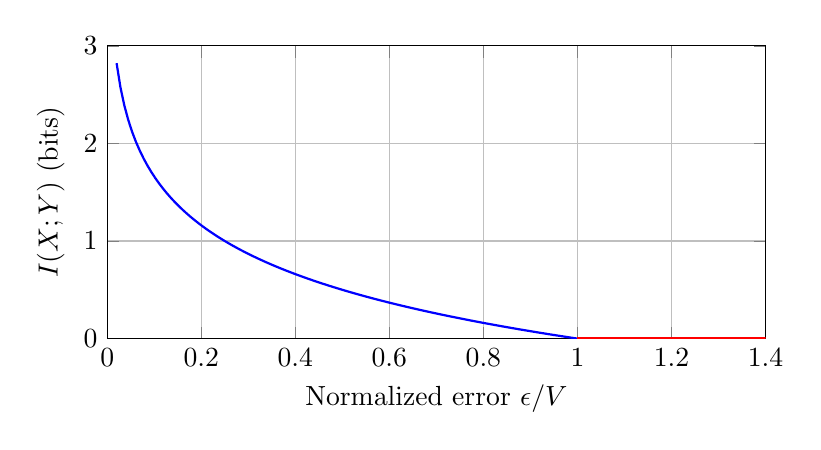
\begin{tikzpicture}
\begin{axis}[width=0.82\linewidth,height=5.3cm,
  xlabel={Normalized error $\epsilon/V$},ylabel={$I(X;Y)$ (bits)},
  xmin=0,xmax=1.4,ymin=0,ymax=3,grid=major]
\addplot+[domain=0.02:1,samples=120,no marks,thick]
  {0.5*ln(1/x)/ln(2)};
\addplot+[domain=1:1.4,samples=2,no marks,thick] {0};
\end{axis}
\end{tikzpicture}
\end{center}
It falls from arbitrarily large information at zero error to zero bits
when we can tolerate error $V$ (just always answer $y=0$).
\end{solution}

\begin{solution}{Problem 4}
Let $\sigma_x^2=\langle x^2\rangle$ and
$\sigma_\xi^2=\langle\xi^2\rangle$. We assume the signal and noise are
independent. Then $\sigma_y^2=g^2\sigma_x^2+\sigma_\xi^2$ and
$\operatorname{Cov}(x,y)=g\sigma_x^2$.

\textbf{(a)} For two jointly Gaussian variables, integrating the Gaussian
log-density ratio gives
$I(X;Y)=-\tfrac12\log_2(1-\rho^2)$, where
\[
 \rho^2=\frac{g^2\sigma_x^2}{g^2\sigma_x^2+\sigma_\xi^2}
        =\frac{S}{1+S}.
\]
Therefore $\boxed{I(X;Y)=\tfrac12\log_2(1+S)}$ bits.

\textbf{(b)} If $Z\sim\mathcal N(0,\sigma^2)$, insert its density into
$h(Z)=-\int p(z)\log_2p(z)\,dz$. Since $\langle Z^2\rangle=\sigma^2$,
\[
 h(Z)=\frac12\log_2(2\pi\sigma^2)
      +\frac{\langle Z^2\rangle}{2\sigma^2\log 2}
      =\boxed{\frac12\log_2(2\pi e\sigma^2)}.
\]
This is differential entropy, so its numerical value depends on the unit
used for $z$.

\textbf{(c)} Given $x$, the only uncertainty in $y=gx+\xi$ is $\xi$.
Consequently,
\begin{align*}
 I(X;Y)&=h(Y)-h(Y|X)=h(Y)-h(\xi)\\
 &=\frac12\log_2\frac{g^2\sigma_x^2+\sigma_\xi^2}{\sigma_\xi^2}\\
 &=\boxed{\frac12\log_2(1+S)}.
\end{align*}
\end{solution}

\begin{solution}{Problem 5}
\textbf{(a)} For narrow one-dimensional bins,
$p_n\simeq P(x_n)\Delta x$. Substitute this in the discrete entropy:
\begin{align*}
 H&=-\sum_n p_n\log_2p_n\\
 &\simeq-\sum_n P(x_n)\Delta x\log_2P(x_n)
        -\log_2(\Delta x)\sum_n p_n\\
 &\longrightarrow S_{\rm continuum}-\log_2(\Delta x).
\end{align*}
In $D$ dimensions, a box has volume $(\Delta x)^D$, giving
$\boxed{H\simeq h_D-D\log_2(\Delta x)}$. The coefficient of
$-\log_2\Delta x$ is the effective dimension.

\textbf{(b,c)} I assigned each of the million points in each file to box
$(\lfloor x/\Delta x\rfloor,\lfloor y/\Delta x\rfloor)$, counted the occupied
boxes, and computed $H=-\sum_{\rm boxes}p\log_2p$. Some results are
\[
\begin{array}{c|rr}
\Delta x&\text{circle}&\text{noisy circle}\\\hline
0.10&5.997&7.227\\
0.05&7.104&9.076\\
0.02&8.440&11.667\\
0.01&9.456&13.647\\
0.005&10.448&15.598\\
0.002&11.760&17.961
\end{array}
\]
\begin{center}
\begin{tikzpicture}
\begin{axis}[width=0.91\linewidth,height=6cm,xmode=log,
  xlabel={$1/\Delta x$},ylabel={Box entropy (bits)},grid=major,
  legend style={at={(0.02,0.98)},anchor=north west}]
\addplot+[mark=*] table[x expr=1/\thisrow{width},y=clean,col sep=comma]{pset2_entropy.csv};
\addlegendentry{Circle}
\addplot+[mark=square*] table[x expr=1/\thisrow{width},y=noisy,col sep=comma]{pset2_entropy.csv};
\addlegendentry{Noisy circle}
\end{axis}
\end{tikzpicture}
\end{center}
For the clean circle, halving the box width adds about one bit at the finer
scales: it is effectively one-dimensional. For the noisy circle, halving
$0.02$ to $0.01$ adds $1.98$ bits and halving again adds $1.95$ bits:
at scales below the noise width the points fill a two-dimensional band.
At larger boxes the ring still looks closer to one-dimensional. At the
very smallest boxes the finite million-point sample starts to cap the
measured entropy at $\log_2(10^6)\simeq19.93$ bits, so that endpoint should
not be used to estimate the dimension.
\end{solution}

\begin{solution}{Problem 6}
The file has $h=7,54,544$ heads in its first $n=10,100,1000$ flips.
Ignoring the common binomial coefficient, the likelihood is
$L(p)=p^h(1-p)^{n-h}$. I maximized its log plus the log of each prior
over $0\leq p\leq1$. For the uniform prior, the derivative
$h/p-(n-h)/(1-p)=0$ gives $\widehat p=h/n$.

For the Gaussian prior, solve
\[
 \frac hp-\frac{n-h}{1-p}-\frac{p-0.5}{0.04}=0.
\]
For the bimodal prior, I evaluated
\[
 h\log p+(n-h)\log(1-p)
 +\log\!\left[\frac1{1+25p^2}+\frac1{1+25(1-p)^2}\right]
\]
on a grid with spacing $10^{-5}$. The resulting MAP estimates are
\[
\begin{array}{c|r|rrr}
n&h&\text{uniform}&\text{Gaussian}&\text{bimodal}\\\hline
10&7&0.70000&0.62617&0.77090\\
100&54&0.54000&0.53766&0.54175\\
1000&544&0.54400&0.54373&0.54418
\end{array}
\]
The prior matters most with only ten flips; after a thousand, the data
mostly decide. For the delta prior, all three samples contain both heads
and tails. Both allowed values, $p=0$ and $p=1$, assign probability zero
to those mixed results. The posterior normalizing constant is therefore
zero: \emph{no MAP estimate exists} under that prior for these data.
\end{solution}

\begin{solution}{Problem 7}
Write $M$ for the mother reading, $U,V$ for the daughters, and define
$T=U+V$ and $D=U-V$. If each surviving molecule contributes brightness
$f$, and a molecule chooses daughter 1 with probability $q_p$, then,
with $r=2q_p-1$,
\[
 E[D\mid T]\simeq rT,\qquad
 E[(D-rT)^2\mid T]\simeq fT(1-r^2).
\]
That second equation is the useful counting-noise signal: it separates
single-molecule brightness from the much larger variation in cell sizes.
I estimated $r=\sum D/\sum T$ and, when readout noise was negligible,
used $\widehat f=\operatorname{mean}[(D-rT)^2/T]/(1-r^2)$.
For degradation, I estimated the surviving fraction from the
through-origin slope $s=\sum MT/\sum M^2$.

\textbf{(a)} The file has 999 numeric rows after its header. It gives
$s\simeq1$, $r\simeq0$, and
$\boxed{f=40.5\pm1.8}$ fluorescence units per protein.
The $\pm$ value is a bootstrap standard error from 1,000 resamples of cells.
The near equality $M\simeq U+V$ agrees with negligible decay and accurate
measurement.

\textbf{(b)} The 1,000 rows give $s\simeq1$ but $r=0.4194$, so the average
daughter share is $q_p=(1+r)/2\simeq0.7097$. Accounting for this uneven
split gives $\boxed{f=23.1\pm1.1}$ units per protein (bootstrap standard
error). Ignoring the unequal split would mistake the systematic daughter
difference for molecular counting noise.

\textbf{(c1)} Here $s=0.8800\pm0.0004$, meaning roughly 12\% of the
mother's fluorescence does not survive to the daughters. The partition
estimate is $\boxed{f=46.6\pm2.0}$ units per protein. Decay explains much
of the failure of $M=U+V$; that failure alone is not evidence of a bad
measurement.

\textbf{(c2)} Here $s=0.9792\pm0.0007$, about 2\% loss, but there is also
substantial additive readout noise. A direct $D^2/T$ calculation gives
about 89 units, which is inflated. I instead fit
\[
 (D-rT)^2\simeq fT+2\sigma_{\rm read}^2
\]
across cells. Its fitted slope gives $\boxed{f=20.3\pm4.0}$ units per
protein, and its intercept $1.03\times10^6$ implies a daughter-readout
standard deviation of roughly $720$ fluorescence units if the two daughter
errors are independent and have equal variance. The uncertainty on $f$
is again a bootstrap standard error. This estimate relies on the assumed
additive, cell-size-independent noise model, so it is less secure than
the first three.
The accompanying \texttt{pset2\_analysis.py} reproduces the calculations
and plots with NumPy (seeds 286 and 198). An AI assistant wrote that code
and these solutions in response to the request to complete the practice
set, show the work in LaTeX, use grey boxes, and compile the document.
\end{solution}

\end{document}
